\documentclass[twocolumn]{myarticle}

\usepackage{mymacros}
\usepackage{parskip}
\usepackage{hyperref}
\usepackage{listings}
\usepackage{booktabs}

\lstset{%
basicstyle=\small\ttfamily,
columns=flexible,
breaklines=true,
numbers=left,
stepnumber=1,}

\newcommand{\mat}[1]{\begin{bmatrix}#1\end{bmatrix}}

\begin{document}

\title{Monte Carlo methods in computational physics}
\author{Casey Daniel and Chris Deimert}
\date{\today}

\maketitle

\section{Introduction}
\label{sec:introduction}

In this report, we explore a number of Monte Carlo numerical methods.
Monte Carlo methods use pseudorandom numbers to explore complicated systems.
These methods tend to converge slowly for simple problems, but can be very efficient for complex problems: especially those with a large number of variables.

In Section~\ref{sec:pseudo_random_numbers}, we look at methods for generating pseudo-random numbers.
These are at the core of any Monte Carlo method.
In Section~\ref{sec:radiative_transfer}, we apply Monte Carlo methods to a real physics problem: photons moving through a slab of material.
In Section~\ref{sec:markov_chain_monte_carlo}, we look at a classic Markov Chain example: a string of sunny and rainy days in which the weather of the next day depends on the weather of the current day.
In Section~\ref{sec:metropolis_hastings_sampling}, we use another Markov Chain method: the Metropolis-Hastings random walk.
This allows us to generate samples from complicated probability distribution functions.
In Section~\ref{sec:simulated_annealing}, we use the simulated annealing algorithm to find the global maxima of functions.
The simulated annealing algorithm is a robust method for finding global maxima of complicated functions.

\section{Pseudo random numbers}
\label{sec:pseudo_random_numbers}

Monte Carlo methods typically rely heavily on our ability to generate a large quantity of random numbers.
We cannot, of course, generate truly random numbers on a deterministic computer, so we have to approximate them with pseudo-random numbers (PRN's).
Having a reliable PRN generator is thus a key prerequisite to any Monte Carlo method.
In this section, we will study the linear congruential method (LCM) for generating PRN's.
The LCM generates a sequence of pseudo-random integers with the $ n $th integer given by
\begin{align}
    I_{n} &= \left( A I_n + C \right) \! \! \! \! \! \mod M
\end{align}
($ I_0 $ is called the "seed".)
We can then generate a sequence $ x_n = I_n/M $ of pseudo-random real numbers with $ 0 < x_n < 1 $.

A Fortran 90 module was created to implement the LCM generator and can be seen in Section~\ref{subsec:pseudo_random_numbers_module}.
This code was tested in a number of ways, the code for which is in Section~\ref{subsec:pseudo_random_numbers_main_code} and Section~\ref{subsec:pseudo_random_numbers_plotting_code}.)

The first, simplest test used $ I_0 = 3 $, $ A = 7 $, $ C = 0 $, and $ M = 10 $.
The result is a repeating sequence of numbers:
\begin{align}
    x &= 0.1, 0.7, 0.9, 0.3, 0.1, 0.7, 0.9, 0.3, \ldots
\end{align}
This sequence repeats after only 4 numbers, demonstrating why small values of $ M $ are a poor choice.
The sequence will repeat after at most $ M $ numbers, so we must select a high value of $ M $ in order to obtain a long sequence (though high values of $ M $ do not \emph{guarantee} a long sequence).

One useful way to test a pseudo-random number generator is to look at the correlation between each generated number and the number that preceded it.
These can be plotted in a 2D scatter plot: patterns on the scatter plot imply that the pseudo-random number generator is actually predictable and thus not very random.
The correlation plots for three different sets of coefficients are shown in Figures \ref{fig:lcm_test_1}, \ref{fig:lcm_test_2}, and \ref{fig:lcm_test_3}.
Note that a seed of $ I_0 = 1 $ was used in each case.
It is found that the third combination of coefficients provides the best pseudo-random number generator.

\begin{figure}[ht!]
    \begin{center}
    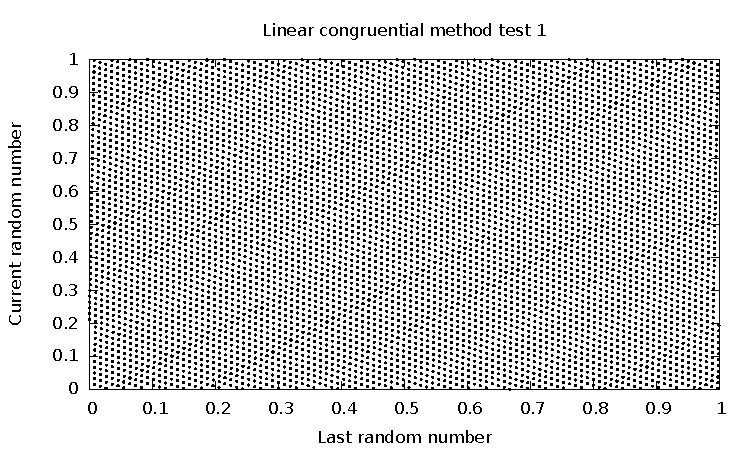
\includegraphics[width = 0.45\textwidth]{../Plots/LCM_test_1.pdf}
    \caption{%
        The correlation plot for $ A = 106 $, $ C = 1283 $, and $ M = 6075 $.
        It is seen that the correlation plot is strongly patterned, meaning that this is a relatively predictable sequence of numbers.
        Thus, this choice of LCM coefficients is a poor one.
    }
    \label{fig:lcm_test_1}
    \end{center}
\end{figure}

\begin{figure}[ht!]
    \begin{center}
    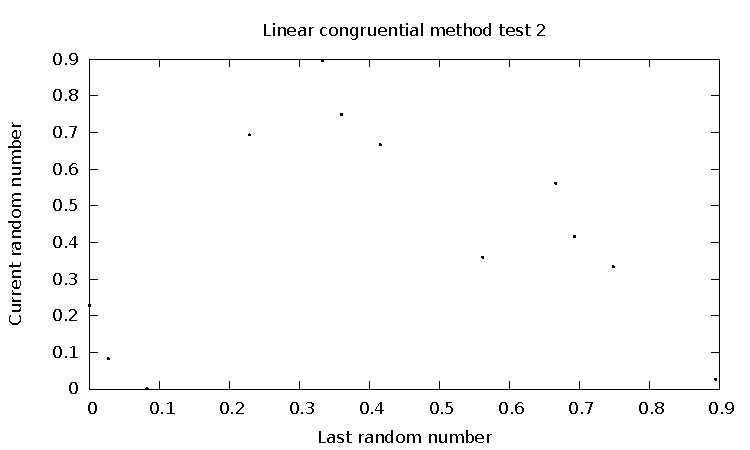
\includegraphics[width = 0.45\textwidth]{../Plots/LCM_test_2.pdf}
    \caption{%
        The correlation plot for $ A = 107 $, $ C = 1283 $, and $ M = 6075 $.
        It is seen that the correlation plot is even more strongly patterned than the last one.
        Thus, this is a relatively predictable sequence of numbers and this choice of LCM coefficients is poor.
        This also demonstrates how small changes in the coefficients lead to drastic changes in the effectiveness of the LCM generator.
        (The coefficients here are the same as the last set except that $ A $ has been increased by 1).
    }
    \label{fig:lcm_test_2}
    \end{center}
\end{figure}

\begin{figure}[ht!]
    \begin{center}
    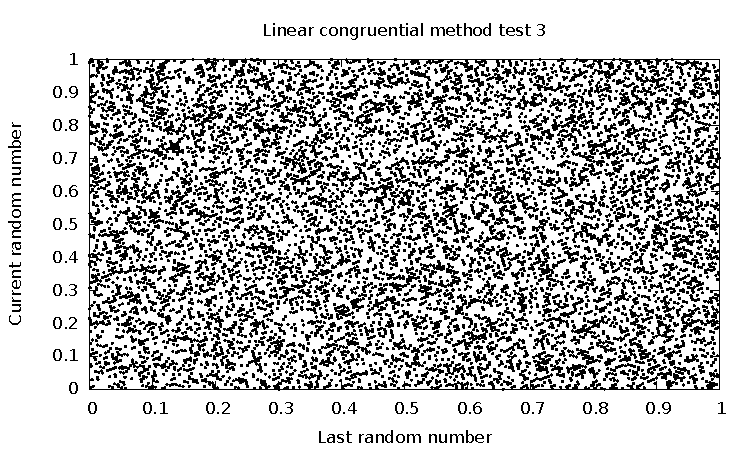
\includegraphics[width = 0.45\textwidth]{../Plots/LCM_test_3.pdf}
    \caption{%
        The correlation plot for $ A = 1103515245 $, $ C = 12345 $, and $ M = 32768 $.
        It is seen that the correlation plot is very weakly patterned, meaning that this is a relatively unpredictable sequence of numbers.
        Thus, this choice of LCM coefficients is a good one.
    }
    \label{fig:lcm_test_3}
    \end{center}
\end{figure}

Another test of pseudo-random number generators that can be performed is a $ \chi^2 $ test.
This is used to determine our statistical confidence in the fact that the pseudo-random numbers are evenly generated.

Using the LCM generator with a seed of $ I_0 = 1 $ and coefficients from the third test above, 100 numbers were generated.
Similarly, 100 numbers were generated using the gfortran generator with a seed based on the computer time.
The distribution of results are shown below.

\bigskip
\begin{center}
    \begin{tabular}{ccccc}
        \toprule
        Interval & Upper limit & LCM & gfortran & Exp. \\
        \midrule
        1  & 0.1 &  6 &  6 & 10 \\
        2  & 0.2 & 11 & 16 & 10 \\
        3  & 0.3 & 12 &  9 & 10 \\
        4  & 0.4 &  9 &  6 & 10 \\
        5  & 0.5 & 10 & 11 & 10 \\
        6  & 0.6 &  9 &  5 & 10 \\
        7  & 0.7 &  8 & 12 & 10 \\
        8  & 0.8 & 10 &  9 & 10 \\
        9  & 0.9 & 11 & 13 & 10 \\
        10 & 1.0 & 14 & 13 & 10 \\
        \bottomrule
    \end{tabular}
\end{center}
\bigskip

The $ \chi^2 $ values for the LCM and gfortran generators are:
\begin{align}
    \chi_{\text{LCM}}^2 &= 6.80
    \\
    \chi_{\text{gfortran}}^2 &= 8.40
\end{align}

These were calculated using 
\begin{align}
    \chi^2 &= \sum_{i=1}^{10} \frac{(O_i - E_i)^2}{E_i}
\end{align}
where $ O_i $ is the observed value in the $ i $th row of the table above, and $ E_i $ is the expeced value. 

It should be noted that the $ \chi^2 $ values change significantly depending on the seed used, though the ones given here are fairly typical.
The LCM $ \chi^2 $ varies from about 2 to about 10, and the gfortran $ \chi^2 $ varies from about 3 to about 18.

In this case, our null hypothesis is that the generated random numbers which are independent and uniformly distributed between 0 and 1.
We have 9 degrees of freedom in this case, which means that the critical $ \chi^2 $ value for 95\% confidence is $ \chi_{\text{crit}}^2 = 16.92 $.
Thus we cannot confidently reject the hypothesis that the pseudo-random number generators are uniformly distributed and independent.

It should be noted that if the number of trials is increased from 100, the $ \chi^2 $ for the LCM decreases while the $ \chi^2 $ for the gfortran remains approximately the same.
We would expect the $ \chi^2 $ to decrease for truly random numbers (from the law of large numbers), so this indicates a problem with the gfortran generator.

A final test we can perform is the auto-correlation test for independence.
The autocorrelation $ A_k $ of a sequence of random variables represents the correlation between the $ t $th number and the $ (t+k) $th random number.
It is given by
\begin{align}
    A_k &= \frac{\displaystyle \sum_{t=1}^{N-k}\big(x_t - \left\langle x \right\rangle\big)\big( x_{t+k} - \left\langle x \right\rangle \big)}{\displaystyle \sum_{t=1}^{N-k} \big( x_t - \left\langle x \right\rangle \big)^2}
\end{align}

The autocorrelation sequences were calculated for both the LCM random generator (with the third set of coefficients) and the gfortran random number generator.
These are plotted in Figure~\ref{fig:lcm_auto_correlation} and Figure~\ref{fig:gfortran_auto_correlation}.

\begin{figure}[ht!]
    \begin{center}
    \includegraphics[width = 0.45\textwidth]{../Plots/LCM_auto_correlation.pdf}
    \caption{%
        The autocorrelation sequence for an LCM generator with $ A = 1103515245 $, $ C = 12345 $, $ M = 32768 $, and $ I_0 = 1 $.
    }
    \label{fig:lcm_auto_correlation}
    \end{center}
\end{figure}

\begin{figure}[ht!]
    \begin{center}
    \includegraphics[width = 0.45\textwidth]{../Plots/Gfortran_auto_correlation.pdf}
    \caption{%
        The autocorrelation sequence for the standard gfortran pseudo-random number generator. 
    }
    \label{fig:gfortran_auto_correlation}
    \end{center}
\end{figure}

We want the autocorrelation to be as close to zero as possible for a pseudo-random number generator.
Small autocorrelations indicate that the random numbers are independent of each other.
It is seen that both generators are pretty good in terms of independence, but the LCM performs slightly better.
The gfortran autocorrelation sequence jumps closer to 1 towards the tail end, indicating a lack of independence.

\section{Radiative transfer}
\label{sec:radiative_transfer}

In this section we apply Monte Carlo methods to the problem of radiative transfer.
Basically, the process is:
\begin{itemize}
\item
    Generate a number of photons at the bottom of a slab.
\item
    Move each photon forward in a random direction by a random distance.
    At each step, there is a probability that the photon is absorbed.
\item
    Repeat until all the photons have either exited the slab or been absorbed.
\end{itemize}

Most random number generators only create numbers uniformly distributed between 0 and 1, so we need to determine how to generate the required random variables in terms of a uniformly distributed random variable $ U $.

First, we look at the optical depth, $ \tau $.
It is exponentially distributed with probability distribution function
\footnote{A note on notation: the prime is used here to distinguish between a random variable ($ \tau $) and the value it takes on ($ \tau' $)}:
\begin{align}
    f_\tau(\tau') &= e^{-\tau'}
\end{align}

The cumulative distribution function is then
\begin{align}
    F_\tau (\tau') &= \int_0^{\tau'} f_\tau (s) d s
    \\
    F_\tau (\tau') &= 1 - e^{-\tau'}
\end{align}

Solving for $ \tau' $, we get
\begin{align}
    \tau' &= - \ln \left( 1 - F_\tau(\tau') \right)
\end{align}

Finally, using the fundamental principle, we find that we can generate optical depths using
\begin{align}
    \tau &= - \ln \left( 1 - U \right)
\end{align}

Note that the actual distance moved by the photon is not $ \tau $, but $ L = \frac{\tau z_\text{max}}{\tau_\text{max}} $, where $ z_\text{max} $ is the thickness of the slab, and $ \tau_\text{max} $ is 20 in this case.
This is shown by:
\begin{align}
    \tau &= \int_0^L n \sigma ds = L n \sigma
\end{align}
and
\begin{align}
    \tau_\text{max} &= \int_0^{z_\text{max}} n \sigma ds = z_\text{max} n \sigma
\end{align}
Dividing the first equation by the second gives
\begin{align}
    L &= \frac{\tau z_\text{max}}{\tau_\text{max}}
\end{align}

When generating random directions, we want to ensure that each differential solid angle $ d \Omega = \sin \theta d \theta d \phi $ is equally likely.
Thus is made easier by defining $ \mu = \cos \theta $ so that $ d \Omega = d \mu d \phi $.
Then, $ \mu $ is a random variable distributed uniformly on $ [-1, 1] $, and $ \phi $ is a random variable distributed uniformly on $ [0, 2\pi] $.
So it is trivial to generate $ \mu $ and $ \phi $ in terms of the unit, uniform random variable $ U $:
\begin{align}
    \mu &= 2U - 1
    \\
    \phi &= 2\pi U
\end{align}
To calculate $ \theta $ we simply use
\begin{align}
    \phi = \cos^{-1} (\mu) = \cos^{-1}(2U-1) 
\end{align}

To test the effectiveness of the fundamental principle, a large number of unit uniform random numbers ($ U $) were generated and used to create distributions of $ \tau $, $ \phi $, $ \mu $, and $ \theta $.
These histograms are shown in Figures~\ref{fig:tau_histogram}, \ref{fig:phi_histogram}, \ref{fig:mu_histogram}, \ref{fig:theta_histogram}.
In each case, $ 10^6 $ trials were run, and the histograms were normalized so that they correspond to an estimated probability distribution function.
In each case, the histogram is exactly as expected, confirming our use of the fundamental principle.

\begin{figure}[ht!]
    \begin{center}
    \includegraphics[width = 0.45\textwidth]{../Plots/Tau_histogram.pdf}
    \caption{%
        Distribution of $ \tau $ generated using a unit uniform random variable $ U $ with the fundamental principle.
    }
    \label{fig:tau_histogram}
    \end{center}
\end{figure}

\begin{figure}[ht!]
    \begin{center}
    \includegraphics[width = 0.45\textwidth]{../Plots/Phi_histogram.pdf}
    \caption{%
        Distribution of $ \phi $ generated using a unit uniform random variable $ U $ with the fundamental principle.
    }
    \label{fig:phi_histogram}
    \end{center}
\end{figure}

\begin{figure}[ht!]
    \begin{center}
    \includegraphics[width = 0.45\textwidth]{../Plots/Mu_histogram.pdf}
    \caption{%
        Distribution of $ \mu $ generated using a unit uniform random variable $ U $ with the fundamental principle.
    }
    \label{fig:mu_histogram}
    \end{center}
\end{figure}

\begin{figure}[ht!]
    \begin{center}
    \includegraphics[width = 0.45\textwidth]{../Plots/Theta_histogram.pdf}
    \caption{%
        Distribution of $ \theta $ generated using a unit uniform random variable $ U $ with the fundamental principle.
    }
    \label{fig:theta_histogram}
    \end{center}
\end{figure}

The final piece needed to perform this Monte Carlo experiment is the absorption probability, which is given in terms of the absorption and scattering cross sections:
\begin{align}
    P_s &= \frac{\sigma_s}{\sigma_s + \sigma_a}
\end{align}
Note that $ P_s $ is between 0 and 1, as expected for a probability.
$ P_s \approx 0 $ for $ \sigma_a \gg \sigma_s $, and $ P_s \approx 1 $ for $ \sigma_a \ll \sigma_s $.

To determine whether a photon is absorbed on a given iteration, we generate a unit uniform random number $ U $. 
The photon scatters if $ U < P_s $ and it is absorbed if $ U > P_s $.

With this setup, a Monte Carlo radiative transfer experiment was run with $ 10^6 $ photons, $ \tau_\text{max} = 10 $, $ z_\text{max} = 1 $ and $ P_s = 1 $ (no absorption).
On this particular run, 101306 photons were transmitted (exited at $ z = z_\text{max} $) and $ 898694 $ were reflected (exited at $ z = 0 $).
It took 532 steps before all photons were either reflected or transmitted.

The orientation of each transmitted photon was captured and put into bins.
This allows us to determine the normalized intensity distribution as a function of $ \theta $ and compare it to the expected theoretical curve.
It is seen in Figure~\ref{fig:scattering_experiment_1} that there is excellent agreement between the theoretical intensity distribution and the distribution calculated using Monte Carlo.

\begin{figure}[ht!]
    \begin{center}
    \includegraphics[width = 0.45\textwidth]{../Plots/Scattering_experiment_1.pdf}
    \caption{%
        Normalized intensity distribution for a radiative transfer experiment with no absorption.
    }
    \label{fig:scattering_experiment_1}
    \end{center}
\end{figure}

A second experiment was performed in which there was 50\% probability of a photon being absorbed at each step ($ P_s = P_a = 0.5 $).
As before, $ \tau_\text{max} = 10 $ and $ z_\text{max} = 1 $.
This time, a much larger number of photons was used: $ 10^8 $.
This was necessary to ensure that enough photons made it through the slab to make an accurate intensity distribution.
Even with $ 10^8 $ incident photons, only 2768 photons were transmitted.
The vast majority (82840816) were absorbed, and the rest (17156416) were reflected.
It took only 28 iterations before all photons were either absorbed, reflected, or transmitted.

The intensity distribution for transmitted photons is shown in Figure~\ref{fig:scattering_experiment_2}.
Not only does the absorption drastically reduce the number of transmitted photons, but it can be seen that absorption also changes the intensity distribution.

\begin{figure}[ht!]
    \begin{center}
    \includegraphics[width = 0.45\textwidth]{../Plots/Scattering_experiment_2.pdf}
    \caption{%
        Normalized intensity distribution for a radiative transfer experiment with absorption ($ P_s = 0.5 $).
    }
    \label{fig:scattering_experiment_2}
    \end{center}
\end{figure}

\section{Markov Chain Monte Carlo}
\label{sec:markov_chain_monte_carlo}

Markov Chains are random processes in which the next state depends only on the current state.
As another example of a Monte Carlo, we perform the classic Markov Chain example: sunny and rainy days.
In this example, the random process is the weather on day $ n $, and we have two possible states for each day: sunny ($ S $) and rainy ($ R $).
The transition probabilities are:
\begin{align}
    P[W_{n+1} = S | W_n = R] &= 0.5
    \\
    P[W_{n+1} = R | W_n = R] &= 0.5
    \\
    P[W_{n+1} = S | W_n = S] &= 0.9
    \\
    P[W_{n+1} = R | W_n = S] &= 0.1
\end{align}
or, in matrix form
\begin{align}
    P &= \mat{0.9 & 0.5 \\ 0.1 & 0.5}
\end{align}

Using this matrix, we can find the probabilities of the next day's weather, given the curent day's weather.
For example, if today is sunny, then the probabilities for tomorrow are
\begin{align}
    \mat{0.9 & 0.5 \\ 0.1 & 0.5} \mat{1 \\ 0} &= \mat{0.9 \\ 0.1}
\end{align}
So given that today is sunny, it is much more likely that tomorrow will be sunny.
Applying the matrix again, we can find the probabilities for two days from now:
\begin{align}
    \mat{0.9 & 0.5 \\ 0.1 & 0.5} \mat{0.9 \\ 0.1} &= \mat{0.86 \\ 0.14}
\end{align}
Again, it is more likely that the day will be sunny.

With Fortran 95 code, we applied the probability matrix repeatedly to two different starting states.
The results are plotted in Figure~\ref{fig:markov_sunny_day} and Figure~\ref{fig:markov_rainy_day}.
It is seen that the probabilities converge towards:
\begin{align}
    P[W_\infty = S] &= 0.833333
    \\
    P[W_\infty = R] &= 0.166667
\end{align}
and the probability matrix after 100 iterations is
\begin{align}
    P^{100} &= \mat{0.833333 & 0.833333 \\ 0.166667 & 1.66667}
\end{align}

\begin{figure}[ht!]
    \begin{center}
    \includegraphics[width = 0.45\textwidth]{../Plots/Markov_Sunny_Day.pdf}
    \caption{%
    Probabilities of sunny and rainy days, given that the first day was a sunny one.
    }
    \label{fig:markov_sunny_day}
    \end{center}
\end{figure}

\begin{figure}[ht!]
    \begin{center}
    \includegraphics[width = 0.45\textwidth]{../Plots/Markov_Rainy_Day.pdf}
    \caption{%
    Probabilities of sunny and rainy days, given that the first day was a rainy one.
    }
    \label{fig:markov_rainy_day}
    \end{center}
\end{figure}

The steady state probabilities are given by:
\begin{align}
    \mat{0.9 & 0.5 \\ 0.1 & 0.5} \mat{P[W_\infty = S] \\ P[W_\infty = R]} &= \mat{P[W_\infty = S] \\ P[W_\infty = R]}
    \\
    \mat{-0.1 & 0.5 \\ 0.1 & -0.5} \mat{P[W_\infty = S] \\ P[W_\infty = R]} &= \mat{0 \\ 0}
\end{align}
which gives
\begin{align}
    P[W_\infty = S] = 5 P[W_\infty = R] 
\end{align}
Choosing values which add up to 1, we get
\begin{align}
    P[W_\infty = S] &= \frac{5}{6} \approx 8.33333
    \\
    P[W_\infty = R] &= \frac{1}{6} \approx 0.16667
\end{align}
which agrees with the predicted results above.

From the numerical results above, we can also guess that
\begin{align}
    P^\infty &= \mat{5/6 & 5/6 \\ 1/6 & 1/6}
\end{align}
and note that
\begin{align}
    \mat{5/6 & 5/6 \\ 1/6 & 1/6} \mat{a \\ b} = \mat{5/6 \\ 1/6}
\end{align}
for any $ a, b $ which add up to 1.
Thus, regardless of the starting condition, the probabilities will always come out to 5/6 and 1/6 in the steady state.
This was confirmed by a number of manual runs of the code.

\section{Metropolis-Hastings sampling}
\label{sec:metropolis_hastings_sampling}

As another example of a Markov-Chain Monte Carlo method, we will use the Metropolis-Hastings random walk.
This can be used to generate samples from complicated probability distributions.
In this case, we will be generating random samples from a distribution proportional to:
\begin{align}
    P(x) &= \frac{1}{2 \sqrt{pi}} \left( \sin 5x + \sin 2x + 2 \right) e^{-x^2}
    \label{eq:p_of_x}
\end{align}

For this implementation of the Metropolis-Hastings algorithm, we will use a normalized distribution centred on the current state.
The proposal distributions are then:
\begin{align}
    q\left(x_n | x^*\right) &= q\left(x^* | x_n\right) = \frac{1}{\sigma \sqrt{2\pi}} \exp \left[\frac{(x^* - x_n)^2}{2\sigma^2}\right]
\end{align}

Our Metropolis-Hastings acceptance probability is
\begin{align}
    \min \left( 1, \frac{p(x^*) q(x^*|x_n)}{p(x_n) q(x_n|x^*)} \right)
\end{align}
However, since $ q(x^*|x_n) = q(x_n|x^*) $, this reduces to
\begin{align}
    \min \left( 1, \frac{p(x^*)}{p(x_n)} \right)
\end{align}
which is the Metropolis criterion.

In general, the inclusion of the ratio allows for non-symmetric proposal probabilities.
If the proposal probability distribution is symmetric (as it is in the case of a normal or uniform distribution centred around the current point), then this ratio is unity and it has no effect.

The key to the Metropolis-Hastings algorithm is the accept-reject step.
We generate a proposed point $ x^* $ using the distribution $ q(x^* | x_n) $.
Then we generate a random variable $ r $ which is uniformly distributed between 0 and 1.
Then the next point $ x_{n+1} $ is given by
\begin{align}
    x_{n+1} &= \begin{cases} x^* & \text{if } r < \min \left( 1, \frac{p(x^*)}{p(x_n)} \right) \\ x_n & \text{otherwise} \end{cases}
\end{align}

Fortran 90 code was created based on this algorithm to sample the distribution $ P(x) $ from Equation~\eqref{eq:p_of_x} above.
This was done using a starting point $ x_0 = 1 $, and different standard deviation values for the proposal distribution: $ \sigma = 0.025, 1.0, 50.0 $.
1000 iterations of the algorithm were run---the results are shown in Figures \ref{fig:metropolis_sigma_025_1000}, \ref{fig:metropolis_sigma_1_1000}, and \ref{fig:metropolis_sigma_50_1000}.
For $ \sigma = 0.025 $, 2.60\% of points were accepted, for $ \sigma = 1 $, 50.0\% of points were selected, and for $ \sigma = 50 $, 98.0\% of points were selected.

It can be seen that $ \sigma = 1 $ gives the best sampling of the distribution.
This is not surprising, since $ P(x) $ is proportional to $ e^{-x^2} $, which has a characteristic length of 1.

\begin{figure}[ht!]
    \begin{center}
    \includegraphics[width = 0.45\textwidth]{../Plots/Metropolis_sigma-025-1000.pdf}
    \caption{%
    Metropolis sampling with $ \sigma = 0.025 $ and 1000 iterations.
    }
    \label{fig:metropolis_sigma_025_1000}
    \end{center}
\end{figure}

\begin{figure}[ht!]
    \begin{center}
    \includegraphics[width = 0.45\textwidth]{../Plots/Metropolis_sigma-1-1000.pdf}
    \caption{%
    Metropolis sampling with $ \sigma = 1 $ and 1000 iterations.
    }
    \label{fig:metropolis_sigma_1_1000}
    \end{center}
\end{figure}

\begin{figure}[ht!]
    \begin{center}
    \includegraphics[width = 0.45\textwidth]{../Plots/Metropolis_sigma-50-1000.pdf}
    \caption{%
    Metropolis sampling with $ \sigma = 50 $ and 1000 iterations.
    }
    \label{fig:metropolis_sigma_50_1000}
    \end{center}
\end{figure}

To improve the sampling, the algorithm was used with the same three $ \sigma $ values, but with 50000 iterations.
The results are shown in Figures \ref{fig:metropolis_sigma_025_50000}, \ref{fig:metropolis_sigma_1_50000}, and \ref{fig:metropolis_sigma_50_50000}.
Overall, the sampling is better in all three cases, however, the $ \sigma = 1 $ test is by far the best.

The acceptance rates for 50000 points were nearly identical to the acceptance rates for 1000 iterations.
For $ \sigma = 0.025 $, 2.12\% of points were accepted, for $ \sigma = 1 $, 50.2\% of points were selected, and for $ \sigma = 50 $, 98.6\% of points were selected.
This shows that the acceptance rate is more strongly controlled by the selection of points than it is by the number of iterations.

\begin{figure}[ht!]
    \begin{center}
    \includegraphics[width = 0.45\textwidth]{../Plots/Metropolis_sigma-025-50000.pdf}
    \caption{%
    Metropolis sampling with $ \sigma = 0.025 $ and 50000 iterations.
    }
    \label{fig:metropolis_sigma_025_50000}
    \end{center}
\end{figure}

\begin{figure}[ht!]
    \begin{center}
    \includegraphics[width = 0.45\textwidth]{../Plots/Metropolis_sigma-1-50000.pdf}
    \caption{%
    Metropolis sampling with $ \sigma = 1 $ and 50000 iterations.
    }
    \label{fig:metropolis_sigma_1_50000}
    \end{center}
\end{figure}

\begin{figure}[ht!]
    \begin{center}
    \includegraphics[width = 0.45\textwidth]{../Plots/Metropolis_sigma-50-50000.pdf}
    \caption{%
    Metropolis sampling with $ \sigma = 50 $ and 50000 iterations.
    }
    \label{fig:metropolis_sigma_50_50000}
    \end{center}
\end{figure}

More tests were run to explore the use of a burn-in phase.
As a control, three tests were run using $ x_0 = -3 $, $ \sigma = 0.2 $ and 1000 iterations.
These results are seen in Figures~\ref{fig:metropolis_burn_1_1}, \ref{fig:metropolis_burn_1_2}, and \ref{fig:metropolis_burn_1_3}.
The acceptance rates were 15.4\%, 16.5\%, and 14.7\%, respectively.

\begin{figure}[ht!]
    \begin{center}
    \includegraphics[width = 0.45\textwidth]{../Plots/Metropolis_burn1-1.pdf}
    \caption{%
    Metropolis sampling with $ \sigma = 0.2 $, 1000 iterations, and no burn-in.
    }
    \label{fig:metropolis_burn_1_1}
    \end{center}
\end{figure}

\begin{figure}[ht!]
    \begin{center}
    \includegraphics[width = 0.45\textwidth]{../Plots/Metropolis_burn1-1.pdf}
    \caption{%
    Metropolis sampling with $ \sigma = 0.2 $, 1000 iterations, and no burn-in.
    }
    \label{fig:metropolis_burn_1_2}
    \end{center}
\end{figure}

\begin{figure}[ht!]
    \begin{center}
    \includegraphics[width = 0.45\textwidth]{../Plots/Metropolis_burn1-1.pdf}
    \caption{%
    Metropolis sampling with $ \sigma = 0.2 $, 1000 iterations, and no burn-in.
    }
    \label{fig:metropolis_burn_1_3}
    \end{center}
\end{figure}

Three more tests were run using $ x_0 = -3 $, $ \sigma = 0.2 $ and 1000 iterations, but this time the first 200 iterations were ignored.
These results are seen in Figures~\ref{fig:metropolis_burn_2_1}, \ref{fig:metropolis_burn_2_2}, and \ref{fig:metropolis_burn_2_3}.
The acceptance rates were 14.4\%, 16.5\%, and 15.0\%, respectively.
It is seen that even though fewer total points are used, the sampling is better when the first 200 iterations are ignored.

\begin{figure}[ht!]
    \begin{center}
    \includegraphics[width = 0.45\textwidth]{../Plots/Metropolis_burn2-1.pdf}
    \caption{%
    Metropolis sampling with $ \sigma = 0.2 $, 1000 iterations, and 200 iteration burn-in.
    }
    \label{fig:metropolis_burn_2_1}
    \end{center}
\end{figure}

\begin{figure}[ht!]
    \begin{center}
    \includegraphics[width = 0.45\textwidth]{../Plots/Metropolis_burn2-1.pdf}
    \caption{%
    Metropolis sampling with $ \sigma = 0.2 $, 1000 iterations, and 200 iteration burn-in.
    }
    \label{fig:metropolis_burn_2_2}
    \end{center}
\end{figure}

\begin{figure}[ht!]
    \begin{center}
    \includegraphics[width = 0.45\textwidth]{../Plots/Metropolis_burn2-1.pdf}
    \caption{%
    Metropolis sampling with $ \sigma = 0.2 $, 1000 iterations, and 200 iteration burn-in.
    }
    \label{fig:metropolis_burn_2_3}
    \end{center}
\end{figure}

\section{Simulated annealing}
\label{sec:simulated_annealing}

Simulated annealing is used to find the global maxima of complicated functions.
It is more robust than traditional hill-climbing techniques at the cost of execution speed.
If $ P(x) $ is the function to be maximized, then the transition probability is
\begin{align}
    A\left(x_n \to x^*\right) &= \min \left( 1, \left( \frac{P\left( x^* \right)}{P \left( x_n \right)} \right)^{1/T_n} \right)
\end{align}

The temperature, $ T_n $, is a key part of this algorithm.
When the temperature is set to 1, then this is simply the Metropolis random walk algorithm.
When $ T_n $ is large (e.g. 100), then the transition probabilities will tend to be high, regardless of $ P(x^*) $ and $ P(x_n) $.
As the temperature ``cools'' down to near unity, the transition probability approaches $ P(x^*)/P(x_n) $ from the Metropolis algorithm.
As the temperature ``cools'' further towards 0, the transition probability approaches a step function: it is 1 if $ P(x^*) > P(x_n) $ and $ 0 $ otherwise.
So for high temperatures, the walk is essentially random, exploring the whole space.
For small temperatures, the walk approaches pure hill-climbing algorithms, narrowing in on local maxima.

Note that if $ P(E) = e^{-E} $, then
\begin{align}
    A\left(x_n \to x^*\right) &= \min \left( 1, e^{(E_n - E^*)/T_n} \right)
\end{align}
Making the replacement $ T_n \to k_B T $ demonstrates why this algorithm is called ``simulated annealing.''
In statistical mechanics, the probability of a transition is proportional to the exponential of the energy difference over $ k_B T $.

The simulated annealing algorithm was implemented by Goffe et al.; this code can be seen in Section~\ref{subsec:simulated_annealing_module_code}.
This code was used to find the maxima of three functions.
We used all the recommended settings for the input parameters, suggested within the Goffe et al.\ code.

The first function
\begin{align}
    f(x,y) &= e^{-\left(x^2 + y^2\right)}
\end{align}
is plotted in Figure~\ref{fig:simulated_annealing_1}.
There is a single maximum at $ (x,y) = (0,0) $.

The simulated annealing found the maximum at
\begin{align}
    (x,y) &= \left( 1.7235 \times 10^{-6}, -4.9737 \times 10^{-6} \right)
\end{align}
which is quite close to the actual value.
The run time, however, was about 43.1 ms, which is quite significant for such a simple task.


\begin{figure}[ht!]
    \begin{center}
    \includegraphics[width = 0.45\textwidth]{../Plots/Simulated_annealing_1.pdf}
    \caption{%
    First function maximized by simulated annealing: $ f(x,y) = e^{-\left(x^2 + y^2\right)} $.
    }
    \label{fig:simulated_annealing_1}
    \end{center}
\end{figure}

The second function
\begin{align}
    f(x,y) &= e^{-\left(x^2 + y^2\right)} 2 e^{-\left( x-1.7 \right)^2 - \left( y - 1.7 \right)^2}
\end{align}
is plotted in Figure~\ref{fig:simulated_annealing_2}.
There is a local maximum at $ (x,y) \approx (0,0) $ and a global maximum at $ (x,y) \approx (1.7, 1.7) $.

The simulated annealing found the maximum at
\begin{align}
    (x,y) &= \left( 1.6973, 1.6973 \right)
\end{align}
which is quite close to the actual global maximum.
So the algorithm did not get fooled by the local maximum like a basic hill-climbing algorithm might.
Again, though, the run time was quite significant at around $ 50.5 $ ms.

\begin{figure}[ht!]
    \begin{center}
    \includegraphics[width = 0.45\textwidth]{../Plots/Simulated_annealing_2.pdf}
    \caption{%
    Second function maximized by simulated annealing: $ f(x,y) = e^{-\left(x^2 + y^2\right)} 2 e^{-\left( x-1.7 \right)^2 - \left( y - 1.7 \right)^2} $.
    }
    \label{fig:simulated_annealing_2}
    \end{center}
\end{figure}

The final function
\begin{align}
    f(x,y) &= (1-x)^2 + 100 (y-x^2)^2
\end{align}
is plotted in Figure~\ref{fig:simulated_annealing_3}.
This time, the simulated annealing algorithm was used to find a global minimum (just a matter of taking the negative of the function).
There is one minimum of this function at $ (x,y) = (1,1) $.

The simulated annealing found the minimum at
\begin{align}
    (x,y) &= \left( 0.99999, 0.99999 \right)
\end{align}
which is quite close to the actual global minimum.
So the algorithm was again successful.
Again, though, the run time was quite significant at around $ 39.5 $ ms.

\begin{figure}[ht!]
    \begin{center}
    \includegraphics[width = 0.45\textwidth]{../Plots/Simulated_annealing_3.pdf}
    \caption{%
    Second function maximized by simulated annealing: $ f(x,y) = (1-x)^2 + 100 (y-x^2)^2 $.
    }
    \label{fig:simulated_annealing_3}
    \end{center}
\end{figure}

Overall, this algorithm is quite robust, but it is computationally expensive.
Simply put, finding the global maximum of a complicated function is going to be hard work.

\section{Conclusions}
\label{sec:conclusions}

In Section~\ref{sec:pseudo_random_numbers}, we looked at methods for generating pseudo-random numbers.
We explored a number of different tests for determining the effectiveness of a pseudo-random number generator.
In Section~\ref{sec:radiative_transfer}, we applied Monte Carlo methods to a real physics problem: photons moving through a slab of material.
Using this method, we were able to generate the intensity distribution as a function of exit angle for a complicated system which is difficult to deal with analytically.
In Section~\ref{sec:markov_chain_monte_carlo}, we looked at a classic Markov Chain example: a string of sunny and rainy days in which the weather of the next day depends on the weather of the current day.
We saw that the system very quickly converges to a probability state which is independent of the original state.
In Section~\ref{sec:metropolis_hastings_sampling}, we used another Markov Chain method: the Metropolis-Hastings random walk.
With this, we were able to generate samples from a very complicated probability distribution function which would have been otherwise difficult to sample from.
In Section~\ref{sec:simulated_annealing}, we used the simulated annealing algorithm to find the global maxima of three functions.
The algorithm was robust and was not fooled by local maxima, but its runtimes were quite long.

\onecolumn

\section{Code}
\label{sec:code}

\subsection{Pseudo random numbers module}
\label{subsec:pseudo_random_numbers_module}

\lstinputlisting[breaklines]{../../Modules/Random_numbers_module.f90}
\vspace{10pt}

\subsection{Pseudo random numbers main code}
\label{subsec:pseudo_random_numbers_main_code}

\lstinputlisting[breaklines]{../Pseudo_RNGs.f90}
\vspace{10pt}

\subsection{Pseudo random numbers plotting code}
\label{subsec:pseudo_random_numbers_plotting_code}

\lstinputlisting[breaklines]{../Pseudo_RNGs.gp}
\vspace{10pt}

\subsection{Radiative transfer code}
\label{subsec:radiative_transfer_code}

\lstinputlisting[breaklines]{../Radiative_transfer.f90}
\vspace{10pt}

\subsection{Radiative transfer plotting code}
\label{subsec:radiative_transfer_plotting_code}

\lstinputlisting[breaklines]{../Radiative_transfer.gp}
\vspace{10pt}

\subsection{Markov chain main code}
\label{subsec:markov_chain_main_code}

\lstinputlisting[breaklines]{../Markov_chain.f90}
\vspace{10pt}

\subsection{Markov chain plotting code}
\label{subsec:markov_chain_plotting_code}

\lstinputlisting[breaklines]{../Markov_chain.gp}
\vspace{10pt}

\subsection{Metropolis main code}
\label{subsec:metropolis_main_code}

\lstinputlisting[breaklines]{../Metropolis.f90}
\vspace{10pt}

\subsection{Metropolis plotting code}
\label{subsec:metropolis_plotting_code}

\lstinputlisting[breaklines]{../Metropolis.gp}
\vspace{10pt}

\subsection{Simulated annealing module code}
\label{subsec:simulated_annealing_module_code}

\lstinputlisting[breaklines]{../../Modules/Simulated_anneal_module.f90}
\vspace{10pt}

\subsection{Simulated annealing main code}
\label{subsec:simulated_annealing_main_code}

\lstinputlisting[breaklines]{../../Presentation/Simulated_anneal_tests.f90}
\vspace{10pt}

\end{document}
